\documentclass[oneside]{VUMIFPSkursinis}
\usepackage{algorithmicx}
\usepackage{algorithm}
\usepackage{algpseudocode}
\usepackage{amsfonts}
\usepackage{float}
\usepackage{amsmath}
\usepackage{bm}
\usepackage{caption}
\usepackage{color}
\usepackage{float}
\usepackage{graphicx}
\usepackage{listings}
\usepackage{subfig}
\usepackage{ltablex}
\usepackage{longtable}
\usepackage{wrapfig}
\usepackage{subfig}
\usepackage{pbox}
\renewcommand{\labelenumii}{\theenumii}
\renewcommand{\theenumii}{\theenumi.\arabic{enumii}.}
\renewcommand{\labelenumiii}{\theenumiii}
\renewcommand{\theenumiii}{\theenumii\arabic{enumiii}.}
\newcolumntype{P}[1]{>{\centering\arraybackslash}p{#1}}
\usepackage[%
	colorlinks=true,
	linkcolor=black
]{hyperref}
\university{Vilniaus universitetas}
\faculty{Matematikos ir informatikos fakultetas}
\department{Programų sistemų katedra}
\papertype{Žmogaus ir kompiuterio sąsaja laboratorinis darbas I}
\title{Alaus gamybos įrangos ir ingredientų pirkimo sistema}
\titleineng{Aludarystės internetinė parduotuvė}
\status{3 kurso studentai}
\author{Greta Pyrantaitė}
\secondauthor{Matas Savickis}
\thirdauthor{Andrius Bentkus}

\supervisor{Kristina Lapin, Doc., Dr.}
\date{Vilnius – \the\year}

\bibliography{bibliografija}

\begin{document}
\maketitle

\sectionnonum{Anotacija}
Šiuo darbu siekiama išanalizuoti ir aprašyti dabartinės www.savasalus.lt sąsajos napatogumus, paaiškinti, koks panaudojimo principas buvo pažeistas, ir šio pažeidimo priežastis.
Šiame darbe taip pat atkreipsime dėmesį į sistemos vartotojų grupes ir jų sąveiką su sitema.
Darbo eigoje apžvelgsime pasisekusias vartotojo sąsajos realizacijas ir aptarsime, kodėl būtent tokie sprendimai yra geresni už esamos sistemos sąsajų realizacijas.

\begin{itemize}
	\item{Greta Pyrantaitė - greta.pyrantaite@gmail.com}
	\item{Matas Savickis - savickis.matas@gmail.com}
	\item{Andrius Bentkus - andrius.bentkus@gmail.com}
\end{itemize}

\tableofcontents

\sectionnonum{Įvadas}
	\subsectionnonum{Programų sistemos ilgasis pavadinimas}
		Alaus gamybos įrangos ir ingredientų pirkimo sistema.
	\subsectionnonum{Programų sistemos trumpasis pavadinimas}
		Aludarystės internetinė parduotuvė
	\subsectionnonum{Dalykinė sritis}
		Elektroninė parduotuvė skirta aludariams.
	\subsectionnonum{Probleminė sritis}
		Sistema turi suteikt galimybę nusipirkti alaus gamybai reikalingus ingredientus ir įrangą bei gauti visą reikalingą informaciją apie ingredientų ir įrangos specifikacijas.
		Sistema taip pat turi vartotojui pateikti informaciją apie alaus gamybos procesą panaudojant nusipirktus ingredientus ir įrangą.
	\subsectionnonum{Naudotojai}
		\begin{itemize}
			\item{Pirkėjas(aludaris) - pirkėjas turi galėti užsisakyti alaus gamybos ingridientus ir įrangą bei gauti reikalingą specifikaciją norint naudotis preke.
				Pirkėjui turi užtekti mokyklinio informatikos kurso žinių ir bendro supratimo, kaip naviguotis internetinėse svetainėse.}
			\item{Pardavėjas - pardavėjui sistema turi suteikti informaciją apie užsakymus, jų apmokėjimus ir panašią svarbią informaciją.
				Sistema pardavėjui taip pat turi suteikti galimybę pridėti arba išimti prekes iš internetinės parduotuvės.
				Pardavėjui taip pat turi užtekti mokyklinio lygio informatikos žinių ir bendrų žinių naviguotis interneto svetainėse.}
		\end{itemize}
	\subsectionnonum{Naudoti dokumentai}
		Kristina Lapin - Žmogaus ir kompiuterio sąveikos paskaitų skaidrės, laboratorinių darbų aprašymai.

\section{Būsimos sistemos įtakojamų asmenų kategorijos}
	\begin{itemize}
		\item{Pirminiai - pirkėjas kuris tiesiogiai naudojasi sistema ir įsigija prekes iš parduotuvės.
			Pardavėjas, kuris paruošia pirkėjo užsakymą.
			Prekių tiekėjas, kurio pelnas didėja nuo pirkėjų skaičiaus.}
		\item{Antriniai - parduotuvės savininkas, kuris gauna statistiką apie prekes ir ruošia personalizuotus užsakymus pirkėjui.}
		\item{Tretiniai - konkurentai (www.aluteksas.lt), kurių pelną ir vartotojų kiekį įtakos mūsų sistemos sėkmė arba nesekmė. }
		\item{Aptarnaujantieji - programuotojai, kuriems teks palaikyti ir ateityje plėsti programų sistemą.}
	\end{itemize}

\section{Pirkėjų grupės poreikiai}
	\subsection{Naudotojų charakteristikos}
		\subsubsection{Informacinių technologijų priemonės}
			Moderni interneto naršyklė, išmanieji telefonai, planšetės, nešiojami kompiuteriai, stacionarūs kompiuteriai.
		\subsubsection{Motyvacija ir galimybės tobulinti įgudžius}
			 Vartotojai, turintys skirtingus informacinių technologijų žinias. 
			Tiek pradedantysis tiek patyręs aludaris gali būti su skirtingom informacinių technologijų žiniom. 
			Vartotojai gali būti su skirtingais fiziniais pajėgumais.
			Gali pasitaikyti vartotojų, kurie parduotuve naudotųsi aukštos drėgmės aplinkoje ir jiems būtų sunkiau naudotis liečiamuoju ekranu.
		\subsubsection{Veiklų kontekstai}
			Vidutinė galimybė gauti pagalbą.
			Vartotojas gali susisiekti su parduotuvės personalu ir pasikonsultuoti dėl pirkinių, tačiau bendru atveju vartotojas atsakymo negaus iš karto.
			Kiekvieno vartotojo poreikiai yra skirtingi, todėl visa bazinė informacija turi būti pateikta parduotuvės puslapyje.
			Svarbu užtikrinti prieigą asmenims su regos ir motoriniais sunkumais.
		\subsubsection{Naudotojų tipas}
			\begin{itemize}
				\item{Naujokas aludaris - Naudotojas pirmą kartą bando išvirti alų, jam reikalingas instruktažas.}
				\item{Patyręs aludaris - Naudotojas ieško specifinių ingridientų ir įrangos pagerinti alaus gamybos procesą ir gaminio kokybę.}
			\end{itemize}
	\subsection{Kompiuterizuojamų veiklų analizė}
		% TODO: remove duplicates
		\subsubsection{Naudotojų charakteristikos}
			\begin{itemize}
				\item{Bendradarbiavimas.}
					Kiekvienu metu bus prisijungę keli vartotojai, tačiau jie tarpusavyje nekomunikuos, todėl jiems ir žinoti vienas apie kitą nereikia.
					Vartotojai komunikuos su pardavėju.
					Ši komunikacija vyks elektroninio pašto pagalba.
				\item{Saugumo kritiškumas.}
					Iš vartotojo pusės sistema nera kritinė.
					Per klaidą būtų įmanoma netyčia nusipirkti kitą prekę arba per daug prekių įsidėti į krepšelį.
					Kaip prevencinė priemonė galėtų būti tai, kad vartotojas prieš atsiskaitydamas už prekes pamatytų visą perkamų prekių sąrašą.
					Per klaidą nusipirkus ne tą prekę vartotojas galėtų informuoti pardavėją.
					Įvykus bet kokiai kitai sisteminiei klaidai, vartotojui būtų parodytas klaidos pranešimas ir jis būtų nukeliamas į pagrindinį langą.
				\item{Turinio ypatumai.}
					Kainos pateikiamos eurais centų tikslumu.
					Datos pateikiamos europiniu formatu(1996-09-21).
					Laikas pateikiamas 24 valandų formatu(21:45).
					Prekės rodomos paveiksliuku su kaina.
			\end{itemize}
	\subsection{Pradedantis aludaris pirmą kartą užsako}
		\subsubsection{Koncepcinis scenarijus}
			Naujokas aludaris - Petrui yra 19 metų ir jis bando išsivirti alų dėl neseniai įvesto Lietuvos sauso įstatymo.
			Petras žino, jog alkoholio akcizas šiuo metu yra labai aukštas ir savo sunkiai uždirbtus pinigus išleisti perkant produktus, turinčius alkoholį, yra ne pats ekonomiškiausias sprendimas.
			Jis nueina į aludarystės internetinę parduotuvę ir bando gauti informaciją apie alaus gamybą namuose.
			Ši informacija nėra lengvai pateikta puslapyje ir Petras ilgai ieško jos, tol kol susiranda pradinuko alaus gamintojo komplektą, kuriame kažkur produkto aprašyme užslėptai yra pridėtas instruktažas.
			Petras įsideda šį komplektą į krepšelį ir nueina į atsiskaitymo formą, kurioje užpildo reikiamą informaciją ir susimoka.
		\subsubsection{Veiklų charakteristikos}
			\begin{itemize}
				\item{Laiko aspektai - Sistemos vartotojas pirmą kartą prisijungti gali tiktais vieną kartą, todėl ši veikla nėra pasikartojanti.
					Tačiau šioje veikloje svarbu, kad vartotojas praeitų visus žingsnius sėkmingai, tam kad įvertintų sistemą tinkama tolimesniam naudojamui, kitom veiklom. }
				\item{Bendradarbiavimas - Vartotojas nesusidurias su kitais vartotojas.
					Vartotojo bendraviams apsiriboja komunikacija su pardavėju kuris gali vartotojui patarti kokias prekes pirti ar pasikonsultuoti dėl gamybos proceso}
				\item{Saugumas - tai nėra kritiška charakteristika vartotojui.
					Svarbu užtikrinti, kad vartotojas nenusipirktų nenorimų prekių.
					Tai bus užtiokrinama jam peržiūrint prekių krepšelį prieš perkant}
				\item{Turinio ypatumai.}
					Kainos pateikiamos eurais centų tikslumu.
					Datos pateikiamos europiniu formatu(1996-09-21).
					Laikas pateikiamas 24 valandų formatu(21:45).
					Prekės rodomos paveiksliuku su kaina.
			\end{itemize}
		\subsubsection{Problemos ir tobulinimo galimybės}
			\begin{itemize}
				\item{Pirminė informacija pradedančiam aludariui yra sunkiai surandama ir neaiškiai pateikta. 
					Vartotojas vidutiniškai užtrunka 2 minutes.}
 				\item{Pirminę informaciją įsisavinti ir nusipirkti tinkamus produktus, atitinkančius ją, yra netriviali užduotis ir svetainė jokiais aspektais nepalengvina šios užduoties. 							Pasiekti norimą rezultatą reikia atlikti daugiau negu 10 veiksmų}
 				\item{Įgyvendinti šį scenarijų užtrunka ilgiau negu 5 minutę, o tai jau yra daugiau negu vidutinis vartotojas turi kantrybės }
			\end{itemize}
		\subsubsection{Būsimasis scenarijus}
			\begin{enumerate}
				\item{Petras nueina į aludarystės internetinę parduotuvę ir bando gauti informaciją apie alaus gamybą namuose}
				\item{Pagrindiniame puslapyje vartotojas paspaudžia ,,PRADEDANTIESIAMS"}
				\item{Atsidaro langas, kuriame pateiktas alaus gaminimo instruktažas teksto forma ir video, demonstruojantis visus reikiamus žingsnius}
				\item{Išvardinti ingridientai yra iš karto pateikti su galimybe įsidėti į krepšelį pačiam instruktaže paminėtas prekes ir nusipirkti jas}
				\item{Petras iš karto įsideda visas reikiamas prekes į krepšelį ir paspaudžia krepšelio piktogramą, kuri atidaro formą, kurioje gali apžiūrėti ir krepšelį, ir užbaigti savo pirkimą}
				\item{Petras dar nė karto nebuvo prisijungęs, todėl turi suvesti papildomus duomenis apie save}
				\item{Petrui pasiūloma užsiregistruoti, tačiau registracija yra neprivaloma}
				\item{Petras nurodo savo apmokėjimo ir kontaktų duomenis, užsakymas yra išsiunčiamas parduotuvės savininkui.}
			\end{enumerate}
		\subsubsection{Panaudojamumo matai ir siekiai}
			\begin{enumerate}
				\item{Nemažiau 90 procentų naujų vartotojų informaciją apie gamybos procesą galės surasti per 1 veiksmą}
				\item{Nemažiau 95 procentai naujas vartotojų prekes iš instruktažo galės įsdėti į krepšelį ne daugiau kaip per 2 veiksmus, įskaitant navigacijos žingsnį į informacijos puslapį}
				\item{100 procentų naujų vartotojų prekes galės nusipirkti neužsiregistravęs į parduotuvę}
				\item{100 procentų naujų vartotojų vaizdo įrašas bus rodomas nereikalaujant atsisiųsti papildomų programų(Flash)}
			\end{enumerate}

	\subsection{Pradedantis aludaris ieško prekės}
		\subsubsection{Koncepcinis scenarijus}
			Naujas aludaris sužino iš savo draugo, kad jam reikia tam tikrų mielių tipo.
			Internetinėje svetainėje dešinėje pusėje vartotojas pamato prekių katalogo meniu juostą.
			Jis spaudžia mygtuką ,,Mielės".
			Puslapis persikrauna.
			Vartotojas meniu juostoje pasirenka mielių tipą.
			Puslapis persikrauna.
			Vartotojas peržiūri visą mielių sąrašą ir pasirenka tas, kurias jam sakė draugas.
			Šio scenarijaus problema yra ta, kad kiekviena kartą paspaudus ant meniu skilties tiklalapis persikrauna.
			Taip pat naujas puslapis kraunasi ilgai, kas trugdo vartotojo patirčiai.
		\subsubsection{Veiklų charakteristikos}
			\begin{itemize}
				\item{Laiko aspektai - pirkėjas pirmą kartą ieško prekės savarankiškai(nesinaudodamas naujoko apmokymais).
					Ateityje ši veikla gali būti pasikartojanti.
					Svarbu, kad pirmą kartą naudojantis prekių paieška meniu būtų pateikta aiškiomis kategorijomis ir neerzintų vartotojų nereikalingais tinklalapio perkrovimais.}
				\item{Bendradarbiavimas - pirkėjas visuomet gali kreiptis į pardavėją norėdamas pasikonsultuoti dėl prekės ieškojimo, bet bendro bendradarbiavimo nebus.}
				\item{Sugumas - šiam scenarijuj papildomas saugumas nereikalingas.
					Svarbu pirkėjui neparodyti prekių, kurios yra išimtos iš prekybos arba kitaip yra nepasiekiamos}
				\item{Turinio ypatimai - meniu pasirinkimai turi būti Lietuvių kalba}
			\end{itemize}
		\subsubsection{Problemos ir tobulinimo galimybės}
			\begin{itemize}
				\item{Kiekvieną kartą paspaudus ant meniu juostos puslapis persikrauna}
				\item{Meniu juostos spalvos per šviesios, todėl sunkiau skaityti meniu sąrašą}
			\end{itemize}
		\subsubsection{Būsimasis scenarijus}
			\begin{enumerate}
				\item{Vartotojas kairėje tiklalapio pusėje pasirenka ,,Mielės"}
				\item{Neperkraunant puslapio atsiskleidžia mielių rūšių pasirinkimas (hamburgeris)}
				\item{Vartotojui pasirinkus norimą mielių rūšį interneto puslapis persikrauna ir vartotojui parodomas visas mielių prekių sąrašas pagal jo parinktą kategoriją}
			\end{enumerate}
		\subsubsection{Panaudojamumo siekiai ir matai}
			\begin{itemize}
				\item{Meniu juostoje pasirinkus kategoriją puslapis nepersikrauna, o atsidaro meniu juosta su kategorijomis}
				\item{Galutinį prekių sąrašą galima pasiekti su maksimaliai vienu puslapio perkrovimu}
				\item{Meniu juostos skiltys yra pavaizduotos kontrastingomis spalvomis ir jas lengva žiūrėti}
				\item{Pasirinkus atitinkamą subkategoriją, prekių sąrašas pasikrauna greičiau negu per 1 sekundę siekiant pagerinti vartotojo patirtį}
			\end{itemize}
	\subsection{Patyrusio aludario prekių ieškojimas}
		\subsubsection{Koncepcinis scenarijus}
			Patyręs aludaris - Matas yra patyręs aludaris, siekiantis įsigyti specialios įrangos ir ingredientų pagerinti alaus gamybos procesą ir pagaminti produkto kokybę.
			Dabartinėje sistemoje ingridientų paieška yra labai paviršutiniška.
			Pavyzdžiui, norėdamas surasti tam tikro rūgštingumo apynių Matas turi atsidaryti apynių skiltį pagrindiniame puslapyje, atsidariusiame naujame lange jis pasirenka apynių tipą.
			Atsidaro langas su visomis prekėmis, kurios yra parduodamos parduotuvėje.
			Parduotuvėje produktų paieškos pagal tam tikrus parametus nėra, taip pat prekių sąraše informacija nenurodyta, todėl Matas, norėdamas surasti tam tikros specifikacijos mielių turi peržiūrėti kiekviną prekę ir skaityti jos aprašymą.
			Tai yra labai nepatogus, daug laiko užimantis ir varginantis procesas.
			Net ir suradus reikiamą produktą neparodomos alternatyvos duotam produktui.
			Tokia pati problema vyrauja ir mielių, salyklo, įrangos bei kitų prekių paieškoje.
		\subsubsection{Veiklų charakteristikos}
			\begin{itemize}
				\item{Laiko aspektai}
					\begin{itemize}
						\item{
							Patyręs aludaris - vartotojas naudojasi sistema 1-2 kartus per mėnesį.
							Šiame scenarijuje vartotojas pats žino, ko ieškoti, todėl jam nereikia prisiminti, kaip kiekvieną kartą vykdyti paiešką.
							Vartotojas turėtų surasti reikiamą prekę per 5 minutes.
							Kiekvienas vartotojas individualiai žino, kokių prekių jam reikia.
						}
					\end{itemize}
			\end{itemize}
		\subsubsection{Problemos ir tobulinimo galimybės}
			\begin{itemize}
				\item{Prekės paieška yra rezultatyvi tuo atveju, jeigu vartotojas tiksliai žino, ko ieško, ir pereina per visas parduotuvėje siūlomas prekes}
				\item{Naudotojui trūksta paieškos galimybių}
				\item{Vartotojui pasirinkus prekę sistema nepasiūlo alternatyvos tai prekei (pvz. pigesnis kito gamintojo variantas)}
			\end{itemize}
		\subsubsection{Būsimasis scenarijus}
			\begin{enumerate}
				\item{Matas nueina į aludarystės internetinę parduotuvę ir bando susirasti reikiamos įrangos ir ingridientų alaus gamybai.}
				\item{Pradiniame puslapyje pirkėjas mato visų turimų prekių kategorijas (įranga, apyniai, salyklas ir t.t.).}
				\item{Vartotojui pasirinkus kategoriją jam parodomas prekių grupės sub-kategorijos.}
				\item{Matas gali tęsti prekės paiešką paspausdamas ant sub-kategorijos piktogramos ir taip išsirinkti norimą prekę arba pasinaudoti prekių paieška, kurioje Matas gali naudotis įvairiais  pasirinkimais ir filtrais, norėdamas rasti konkrečią prekę. Vartotojui taip pat suteikiama galimybė vykdyti paiešką į paieškos laukelį įvedus raktinius žodžius.}
				\item{Nepavykus surasti prekės, paieškos laukelio pagalba Matui yra pasiūlomos panašios prekės pagal laukelio reikšmę.}
				\item{Prekių sąraše prie kiekvienos prekės piktogramos pateikiama trumpa prekės charakteristika. }
				\item{Matas prekes gali išrūšiuoti pagal: kainą, gamintoją, pavadinimą, populiarumą, įvertinimą.}
				\item{Pasirinkus konkrečią prekę parodomas detalus prekės aprašymas, taip pat pateikiamos panašios prekės.}
			\end{enumerate}
	\iffalse
	\subsection{Panaudojamumo siekiai ir matai (TODO: iš čia išimti ir įrašyti į atskirai kiekvienai veiklai)}
		\begin{itemize}
			\item{Patyręs vartotojas konkrečią prekę galės surasti ne daugiau kaip per 5 veiksmus}
			\item{Patyrusiam varototojui bus pateikta detali paieškos sistema}
			\item{Vartotojui bus suteikta galimybė rušiuoti prekes pagal aktualius kriterijus}
			\item{Patyrusiam varotojui prekių saraše bus pateikta trumpa kiekvienos prekės charakteristika}
			\item{Kiekviena prekė turės detalų aprašymą ir naudojimosi instrukciją, jeigu ji yra reikalinga}
			\item{Vartotojui bus suteikta galimybė susisiekti su pardavėju dėl konsultacijos apie prekes}
		\end{itemize}
	\fi
\section{Pardavėjo poreikiai}
	\subsection{Naudotojų charakteristikos}
		\subsubsection{Informacinių technologijų priemonės}
			Moderni interneto naršyklė, nešiojami kompiuteriai, stacionarūs kompiuteriai.
		\subsubsection{Motyvacija ir galimybės tobulėti}
			Pardavėjas bus gerai susipažinęs su parduotuvės sistema. 
			Pardavėjęs turi vidutines informacinių technologijų žinias.
			 Pardavėjęs gali turėti regos sutrikimų (silpna rega).
		\subsubsection{Veiklų kontekstai}
			Pardavėjui reikia sukurti ir pristatyti detalias instrukcijas kaip naudotis sistema, nes po sistemos perdavimo komunikacija su sistemos kūrėjais bus limituotas. Svarbu paruošti instrukciją, kurią galėtų sekti nauji pardavėjai.
		\subsubsection{Naudotojų tipai}
			Pardavėjas - kasdien naudojantis sistemą užsakymams apdoroti.
			Būtų galima išskirti dvi grupes, naujas pardavėjas ir pardavėjas su patirtimi, tačiau įsisavinti sistemą iš pardavėjo pusės neturėtų trukti ilgai.
	\subsection{Kompiuterizuojamų veiklų analizė}

	\subsection{Pardavėjas įvykdo užsakymą}
		\subsubsection{Koncepcinis scenarijus}
			Jonas yra pardavėjas, siekiantis kontroliuoti ir įgyvendinti užsakymus, kuriuos pateikia pirkėjai. Jonas atsidaro pardavėjo sistemą, bet prieiti prie užsakymų reikia per 3 paspaudimus. Galiausiai paspaudus ''Mano užsakymai'', parodomas užsakymų sąrašas, kuriame nurodytas prekės su pavadinimais, adresas ir būsena (apmokėta, neapmokėta, paruošta atsiėmimui, atsiimta). Jonas nori matyti visus neįvykdytus užsakymus puslapio pradžioje, bet tam nėra galimybės. Norint pamatyti daugiau informacijos, reikia paspausti mygtuką ''Rodyti daugiau''.  Surinkus visas nurodytas prekes Jonas pakeičia užsakymo būseną į ''Paruošta atsiėmimui''.

		\subsubsection{Veiklų charakteristikos}
		\begin{itemize}
	\item{Laiko aspektai. Veiklos dažnis  priklauso nuo naudotojo patyrimo: naujokas pardavėjas - kadangi pardavėjas nepatyręs, tikriausiai neturi daug užsakymų, todėl sistema tikėtina nesinaudoja kiekvieną dieną. Svarbus sistemos naudojimosi aiškumas ir patikimumas. Patyręs pardavėjas - tikėtina, kad patyręs pardavėjas naudojasi sistema kiekvieną dieną. Sistema jau turėtų būti perprasta, todėl svarbus našumas, supaprastinta prieiga prie dažnai naudojamų funkcijų.Veiklos trukmė turėtų būti truputį ilgesnė naujam pardavėjui negu patyrusiam, bet iš esmės rasti peržiūrėti informaciją turėtų trukti ne ilgiau nei 5 min. Kadangi pardavėjui svarbu tik peržvelgti informaciją ir ją atnaujinti, veikla nuosekli, o atsako laikas nėra tiek aktualus.}
	\item{Veiklų sudėtingumas. Klaidos nekritiškos, bet neteisingas būsenos atnaujinimas gali sukelti problemų.}
	\end{itemize}
		\subsubsection{Problemos ir tobulėjimo galimybės}
			\begin{itemize}
				\item{Pardavėjui sunku greitai surasti preigą prie savo prekių užsakymų.}
				\item{Užsakymų sąraše neparodyta visa informacija, kuri gali būti reikalinga pardavėjui. Prie jos norint prieiti reikia paspausti dar vieną mygtuką.}
				\item{Pardavėjas negali rūšiuoti užsakymų.}
				\item{Jei kyla netikėtumų ir reikia susisiekti su klientu, reikia tai daryti per parduotuvės atstovus.}
			\end{itemize}

		\subsubsection{Būsimasis scenarijus}
			\begin{enumerate}
				\item{Linas nueina į aludarystės internetinę parduotuvę ir bando gauti informaciją apie užsakymus.}
				\item{Pagrindiniame puslapyje vartotojas paspaudžia ,,Užsakymai"}
				\item{Atsidaro langas, kuriame pateiktas sąrašas su visais užsakymais}
				\item{Užsakyme nurodyta, kokios prekės buvo užsakytos, apmokėjimo būdas, kaina, data, adresas ir užsakymo būsena (apmokėta, neapmokėta, paruošta atsiėmimui, atsiimta)}
				\item{Linas pasirenka dar neparuoštą atsiėmimui užsakymą}
				\item{Linas surenka prekes iš parduotuvės ir paruošia atsiėmimui}
				\item{Pristačius arba vartotojui pačiam atsiėmus prekes, pardavėjas atnaujina užsakymo būseną į ,,Atsiimta".}
				\end{enumerate}
	\subsubsection{Panaudojamumo siekiai ir matai}
		\begin{itemize}
			\item{Pardavėjas savo užsakymų sąrašą galės rasti ne daugiau nei per 2 veiksmus}
			\item{Pardavėjas turi turėti galimybę susisiekti su pirkėju ne daugiau nei per 4 veiksmus}
			\item{Pardavėjas kiekviena prekę galės surasti nedaugiau kaip per 3 veiksmus}
			\item{Pardavėjas turi turėti galimybę pasinaudoti rūšiavimo pagal datą ir būseną funkcija per 5 veiksmus}
			\item{Pardavėjas galės pakeisti būseną ne daugiau nei per 3 veiksmus}
		\end{itemize}

	\subsection{Pardavėjas išima prekes iš prekybos}
		\subsubsection{Koncepcinis scenarijus}
			Jonas nori turėti teisę redaguoti savo prekes. Jonas šiuo metu turi susisiekti su parduotuvės atstovu, kad prekė nebūtų rodoma sąrašuose. Tai labai nepatogu Jonui, taip pat ir jo klientui, nes prekės, kurių nėra sandėliuose, ar, jei jos išvis nebebus siūlomos, yra vis dar rodomos svetainėje. Jonas norėtų turėti galimybę pats pašalinti prekes be tarpininko.
		\subsubsection{Veiklų charakteristikos}
		\begin{itemize}
		\item{Laiko aspektai - prekių išėmimas iš prekybos nėra dažna ar ilgai trunkanti veikla. 
		Viskas vykdoma nuosekliai, nėra daug žingsnių, todėl nebūtina jų saugoti. }
		\item{Veiklų sudėtingumas - veikla determinuota, viskas vyksta pažingsniui.}
		\item{Saugumo kritiškumas - nors klaidos ir sukeltų problemų, jos nėra kritiškos.}
		\end{itemize}
		\subsubsection{Problemos ir tobulinimo galimybės}
			\begin{itemize}
				\item{Pirkėjas mato prekes, kurių negali įsigyti}
				\item{Pardavėjas negali išimti prekių iš prekybos be parduotuvės atstovo patvirtinimo}
				\item{Informacija labai lėtai atnaujinama}
			\end{itemize}
		\subsubsection{Būsimasis scenarijus}
			\begin{enumerate}
				\item{Linas nueina į aludarystės internetinę parduotuvę ir bando išimti prekę iš prekybos.}
				\item{Pagrindiniame puslapyje vartotojas paspaudžia ,,Mano prekės".}
				\item{Atsidaro langas, kuriame pateiktas sąrašas su visomis prekėmis.}
				\item{Prekių sąraše prie kiekvienos prekės piktogramos pateikiama trumpa prekės charakteristika.}
				\item{Linas pasirenka prekę ir ant jos apspaudžia.}
				\item{Linui parodoma visa informacija apie prekę ir mygtukas Redaguoti.}
				\item{Linui paspaudus mygtuką Redaguoti atsiranda pasirinkimas išimti prekę iš prekybos.}
				\item{Išėmus prekę iš prekybos, Linas grąžinamas į visų prekių sąrašą.}
			\end{enumerate}
		\subsubsection{Panaudojamumo siekiai ir matai}
			\begin{itemize}
				\item{Pardavėjas galės išimti prekę iš prekybos ne daugiau nei per 5 veiksmus.}
				\item{Pardavėjas prekių redagavimo funkcionalumą galės atlikti ne daugiau nei per 7 veiksmus}
			\end{itemize}
\section{Įkvepiančios esamų interfeisų idėjos}
	\subsection{Paieškos interfeisas}
		\begin{figure}[h]
			\centering
			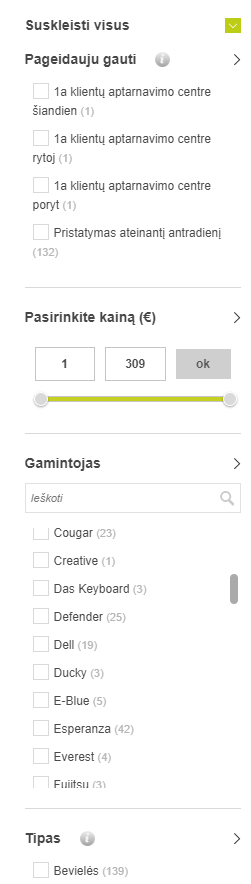
\includegraphics[width=6cm,height=18cm,keepaspectratio]{IkvepiantisInterfeisas1.png}
			\caption{ Paieška}
		\end{figure}

		Šis interfeiso pavyzdys(1 pav.) yra paimtas iš www.1a.lt internetinės parduotuvės prekių paieškos.
		Vartotojas gali pasirinkti paieškos kriterijus paspausdamas ,,check box" mygtukus, kriterijai gali būti sumažinami siekiant lengviau peržiūrėti visų kriterijų sąrašą.
		Šią interfeiso idėją būtų galima perpanaudoti alaus įrangos ir ingridientų paieškai mūsų sistemoje.
	\pagebreak
	\subsection{Prekės charakteristikos interfeisas}
		\begin{figure}[h]
			\centering
			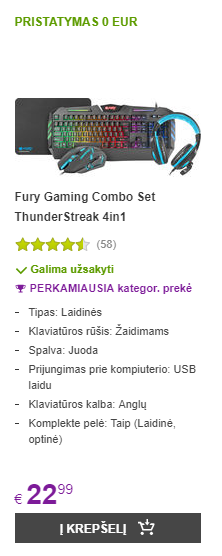
\includegraphics[width=6cm,height=18cm,keepaspectratio]{IkvepiantisInterfeisas2.png}
			\caption{ Prekės charakteristikos}
		\end{figure}
		 Dar vienas interfeiso pavyzdys iš www.1a.lt. 2 pav.
		 paveikslėlyje parodyta, kaip atrodo trumpas prekės aprašymas visų prekių sąraše.
		 Šią idėją galima perpanaudoti rodant prekių informaciją aludarystės parduotuvėje.
		 Igyvendinus šį interfeisą vartotojui nereiktų atsidarinėti kiekvienos prekės puslapio, norint sužinoti bazinę informaciją.
		\pagebreak
	\subsection{Siūlomų panašių prekių interfeisas}
		\begin{figure}[h]
			\centering
			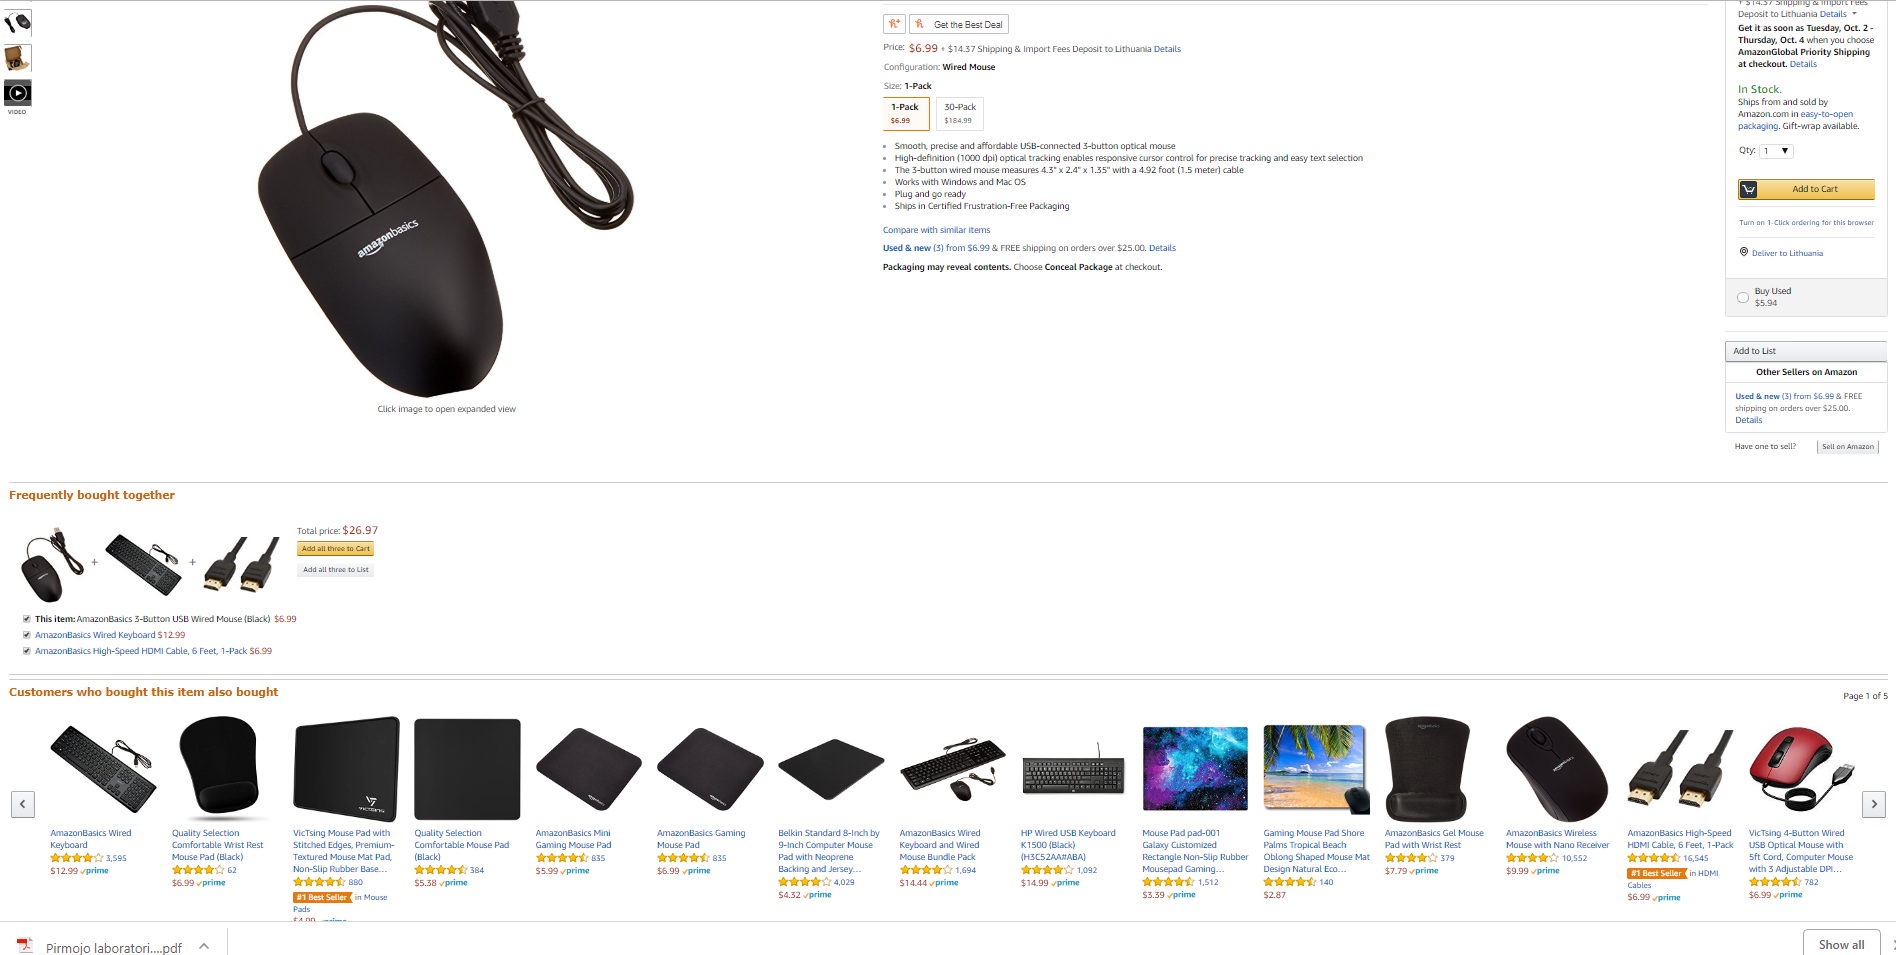
\includegraphics[width=15cm,height=18cm,keepaspectratio]{IkvepiantisInterfeisas3.png}
			\caption{ Prekės charakteristikos}
		\end{figure}

		Šiame pavyzdyje(3 pav.) pateikiamas www.amazon.com interfeiso sprendimas, rodantis prekes, kurias pirko kiti vartotojai, kurie taip pat pirko prekę, kurią vartotojas apžiūri(Customers who bought this item also bought).
		Šią idėją galima perpanaudoti aludarystės sistemoje parodant vartotojui panašias ir/ar pigesnes prekes į tą prekę, kurią vartotojas dabar apžiūri.

		\pagebreak
	\subsection{Interfeisas naujiems vartotojams}
		\begin{figure}[h]
			\centering
			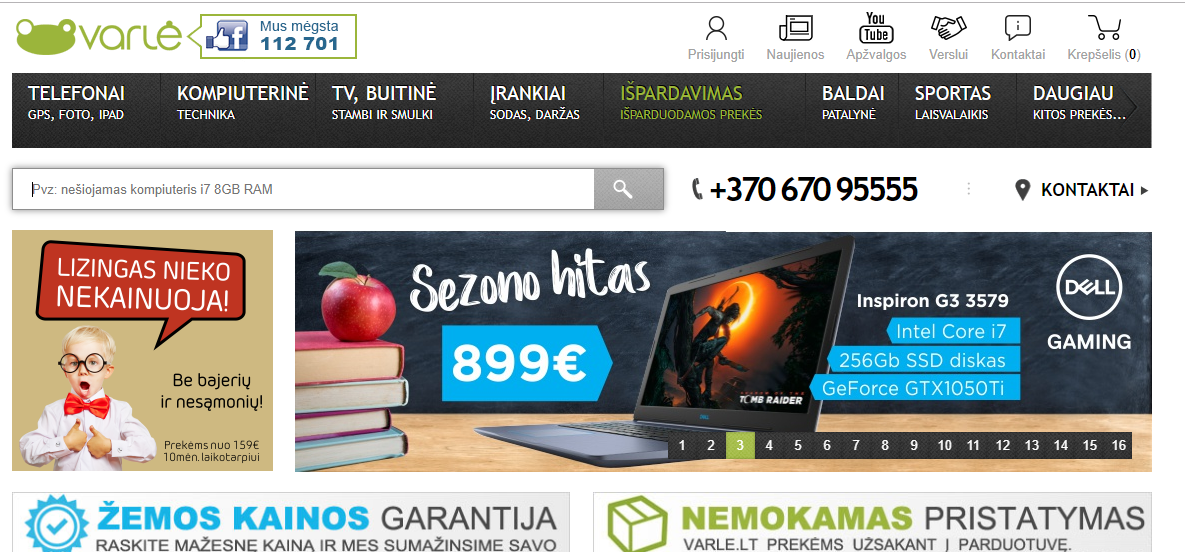
\includegraphics[width=15cm,height=18cm,keepaspectratio]{IkvepiantisInterfeisas4.png}
			\caption{ Prekės charakteristikos}
		\end{figure}

		Paimtas interfeiso pavyzdys(4 pav.) iš internetinės parduotuvės www.varle.lt.
		Žmonės labiau linkę pirkti prekes su nuolaida negu be jos, todėl pirmas dalykas, kurį žmogus pastebi, yra didelis žalias mygtukas ,,IŠPARDAVIMAS".
		Šią dėmesio patraukimo idėją būtų galima pritaikyti atkreipiant naujų aludarių dėmesį nuo ko pradėti.
		Aludarystės parduotuvės viršuje padaryti didelį ryškų mygtuką ,,PRADEDANTIESIAMS" ar kažką panašaus atkreipiant naujų aludarių dėmesį.
		\pagebreak
	\subsection{Atsiskaitymo interfeisas}
		\begin{figure}[h]
			\centering
			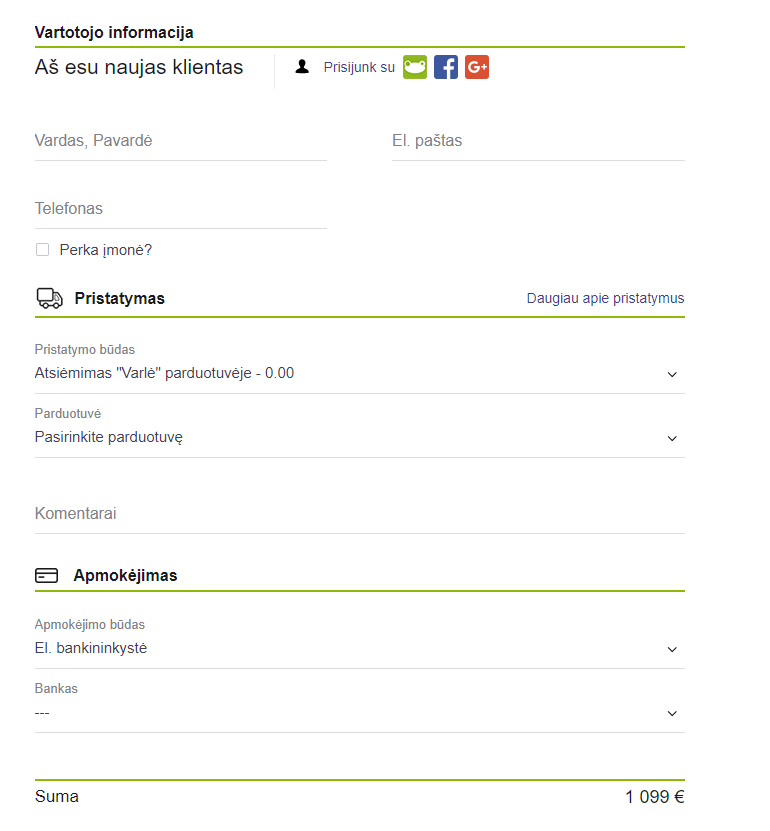
\includegraphics[width=12cm,height=18cm,keepaspectratio]{IkvepiantisInterfeisas5.png}
			\caption{ Prekės charakteristikos}
		\end{figure}

		Šiame pavyzdyje (5 Pav.) matome www.varle.lt interfeiso sprendimą atsiskaitant už prekes.
		Už prekes galima atsiskaityti nesiregistruojant, prie parduotuvės galima prisijungti su Facebook arba Google paskyra, kuri po prisijungimo užpildys dalį duomenų, reikalingų prekės užsakymui, ir pati atsiskaitymo forma yra trumpa, aiški, visa informacija pateikiama viename lange.
		Įgyvendinus šio interfeiso idėją aludarystės parduotuvėje vartotojas galėtų atsiskaityti už prekes greičiau.

%\section{Terminų žodynėlis}
%\section{Priedai}

\end{document}
